\documentclass[spanish,aspectratio=169]{beamer}
\usepackage[utf8]{inputenc}
\usepackage[T1]{fontenc}
\usepackage[spanish,es-tabla]{babel}
\usepackage[scaled=.96]{helvet}
\usepackage{graphicx,booktabs,tikz}
\usetikzlibrary{babel}
\renewcommand{\familydefault}{\sfdefault}
\definecolor{itescaRedDark}{HTML}{8F1117}
\definecolor{itescaCharcoal}{HTML}{141414}
\definecolor{itescaPaper}{HTML}{F7F7F7}
\definecolor{itescaMuted}{HTML}{666666}
\setbeamertemplate{navigation symbols}{}
\setbeamercolor{normal text}{fg=itescaCharcoal,bg=white}
\setbeamercolor{structure}{fg=itescaRedDark}
\setbeamercolor{frametitle}{fg=white,bg=itescaCharcoal}
\setbeamercolor{block title}{fg=white,bg=itescaRedDark}
\setbeamercolor{block body}{fg=itescaCharcoal,bg=itescaPaper}
\setbeamerfont{frametitle}{size=\large,series=\bfseries}
\setbeamersize{text margin left=.6cm,text margin right=.6cm}
\setbeamertemplate{footline}{\hbox{\begin{beamercolorbox}[wd=\paperwidth,ht=2.7ex,dp=1ex,leftskip=.6cm,rightskip=.6cm]{frametitle}\scriptsize M. J. de la Cruz\hfill Plan de Negocios -- ITESCA\hfill\insertframenumber/\inserttotalframenumber\end{beamercolorbox}}}
\graphicspath{{ITESCA/maestria-en-gestion-administrativa/plan-de-negocios-mga/assets-plan-de-negocios/}}
\newenvironment{contenido}{\begin{minipage}{.77\textwidth}\raggedright}{\end{minipage}\hfill}
\newcommand{\fuente}[1]{\par\medskip{\scriptsize\color{itescaMuted}#1\par}}
\hypersetup{hidelinks,pdftitle={AM Taller Autocentro: Presentacion del plan de negocios},pdfauthor={Martin Jonathan de la Cruz Munoz}}
\begin{document}

\begin{frame}{AM Taller Autocentro}
\begin{contenido}
\begin{columns}[c,onlytextwidth]
\begin{column}{.32\linewidth}

\includegraphics[width=\linewidth]{am-taller-logo-1024.png}
\end{column}
\begin{column}{.62\linewidth}
{\Large\bfseries Atención automotriz con autorización y trazabilidad}\par\medskip
Martín Jonathan de la Cruz Muñoz\par
{\small Maestría en Gestión Administrativa\par Plan de Negocios -- Actividad 15\par Docente: Celia Velázquez Reyna\par Monterrey, Nuevo León\par 12 de octubre de 2026}
\end{column}
\end{columns}
\medskip
\includegraphics[height=.6cm]{ITESCA/assets-itesca/web/logo-itesca-contorno.png}
\end{contenido}
\end{frame}

\begin{frame}{El negocio: claridad antes de intervenir}
\begin{contenido}
\begin{block}{Servicio inicial de referencia}
Cambio de aceite y filtro para vehículos ligeros, conforme a las especificaciones de su fabricante.
\end{block}
\begin{itemize}
\item Alcance e importe explicados antes del trabajo cobrable.
\item Orden, autorización, ejecución y cierre documentados.
\item Mecánica, llantas y refacciones: líneas previstas, no inclusiones automáticas.
\end{itemize}
\textbf{Misión:} atención confiable, comunicación clara y ejecución autorizada.\par\medskip
\textbf{Visión:} consolidación local durante cinco años desde el inicio, condicionada a demanda y recursos.
\fuente{Diseño propio de AM Taller. Marco: Laverty y Littel, Entrepreneurship, sección 11.4.}
\end{contenido}
\end{frame}

\begin{frame}{Monterrey: contexto no equivale a compradores}
\begin{contenido}
\begin{columns}[T,onlytextwidth]
\begin{column}{.48\linewidth}
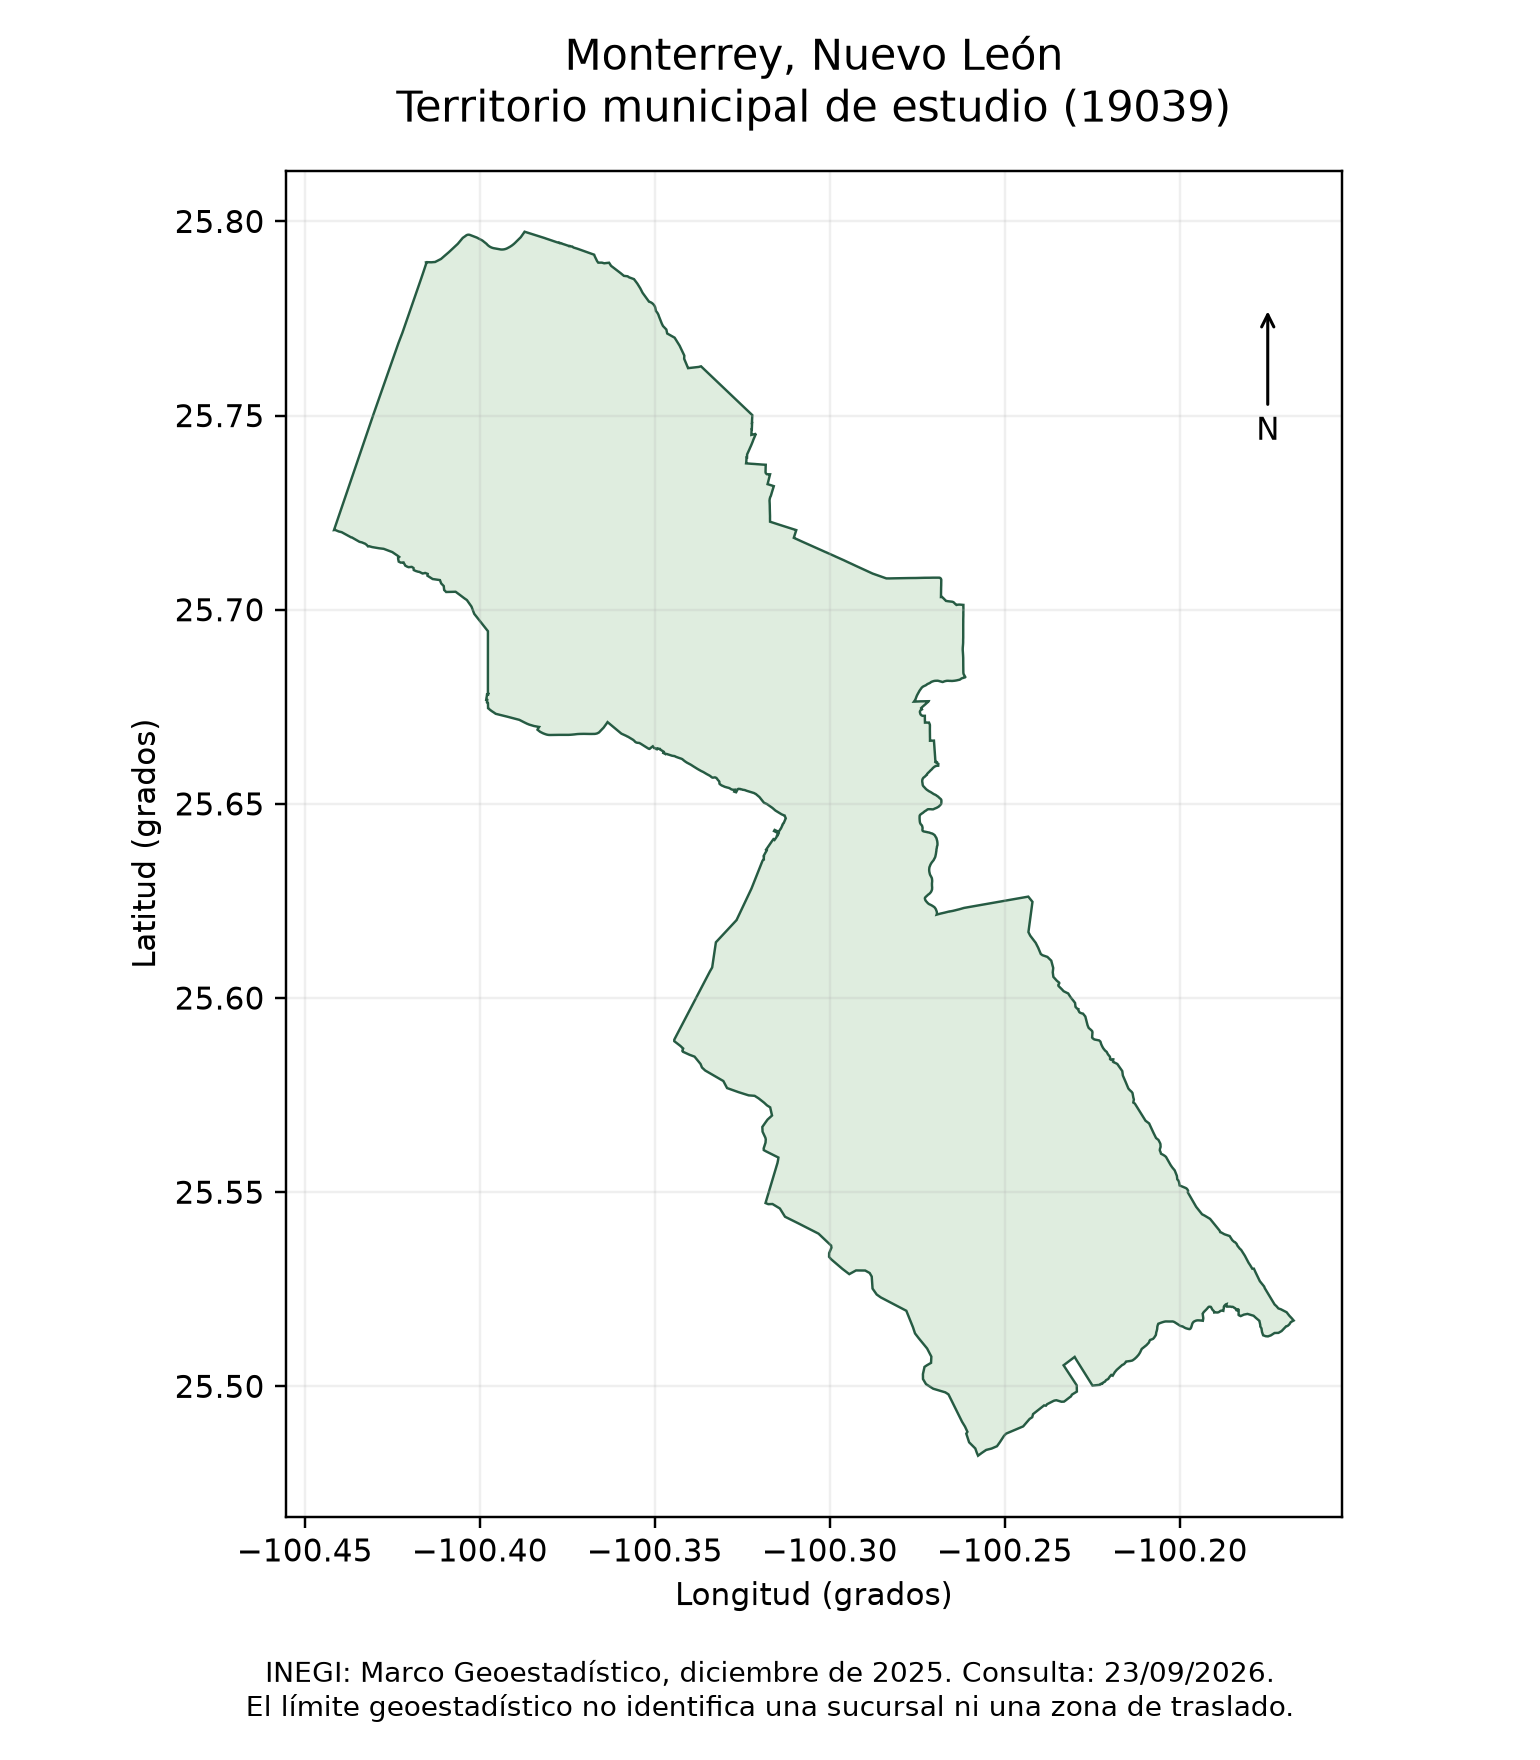
\includegraphics[height=4.6cm]{mapa-monterrey-inegi.png}
\end{column}
\begin{column}{.47\linewidth}
{\Large\bfseries 1,142,994}\par habitantes, Censo 2020\par\medskip
{\Large\bfseries 329,095}\par viviendas habitadas\par\medskip
Cliente objetivo: persona adulta que decide servicios para un vehículo ligero.\par\medskip
\textbf{Domicilio operativo pendiente.}
\end{column}
\end{columns}
\fuente{INEGI: municipio 19039, Censo 2020; Marco Geoestadístico, diciembre de 2025. No son estimaciones de compradores ni cifras actualizadas a 2026.}
\end{contenido}
\end{frame}

\begin{frame}{Mercado: instrumentos listos, sondeo pendiente}
\begin{contenido}
\begin{block}{22 preguntas de demanda + 16 ítems de oferta}
Servicio, frecuencia, gasto y satisfacción; categorías, horarios, condiciones y precios comparables.
\end{block}
\begin{itemize}
\item D07--D11: experiencia de servicio y gasto con alcance identificado.
\item O01--O16: cada observación requiere fecha y fuente.
\item Sondeo por conveniencia en Monterrey; respuestas voluntarias y anonimizadas.
\end{itemize}
\textbf{No hay base de respuestas ni fichas verificadas de oferentes.}\par\medskip
No se afirma demanda suficiente, preferencia por la marca ni superioridad comprobada.
\fuente{Instrumentos propios. Gomez Albrecht, Green y Hoffman (2023), Principles of Marketing, sección 6.3.}
\end{contenido}
\end{frame}

\begin{frame}{Metas a cinco años y riesgos de diseño}
\begin{contenido}
{\small\begin{tabular}{@{}lrrrrr@{}}\toprule
Año desde inicio & 1 & 2 & 3 & 4 & 5\\\midrule
Servicios meta & 360 & 450 & 540 & 630 & 720\\
Clientes distintos & 240 & 300 & 360 & 420 & 480\\\bottomrule
\end{tabular}}\par\medskip
\textbf{Supuestos:} 1.5 servicios por persona; capacidad hipotética de 900 servicios equivalentes al año. No son ventas o capacidad medidas.\par\medskip
\begin{itemize}
\item Fortaleza prevista: registros y controles de autorización.
\item Debilidad actual: faltan sondeo, costos y recursos comprobados.
\item Oportunidad por contrastar: atención clara valorada por usuarios.
\item Amenazas por examinar: competencia e insumos variables.
\end{itemize}
\fuente{Escenarios propios del integrador; estación y tiempos productivos hipotéticos. No se suman clientes como captación acumulada.}
\end{contenido}
\end{frame}

\begin{frame}{Identidad: compromiso convertido en control}
\begin{contenido}
\begin{columns}[c,onlytextwidth]
\begin{column}{.42\linewidth}

\includegraphics[width=\linewidth]{am-taller-logo-1024.png}
\end{column}
\begin{column}{.53\linewidth}
{\Large\bfseries Pasión por los autos.\par Compromiso contigo.}\par\medskip
Autoría propia confirmada.\par\medskip
La promesa se expresa en presupuesto, autorización y cierre.\par\medskip
No acredita registro de marca ni preferencia del consumidor.
\end{column}
\end{columns}
\fuente{Logotipo propio, confirmado el 23 de septiembre de 2026.}
\end{contenido}
\end{frame}

\begin{frame}{Publicidad: piloto limitado y medible}
\begin{contenido}
\begin{columns}[c,onlytextwidth]
\begin{column}{.43\linewidth}

\includegraphics[height=5.2cm]{flyer-am-taller-propuesta.png}
\end{column}
\begin{column}{.52\linewidth}
\textbf{Piloto propuesto: 30 días}\par\medskip
Volantes y difusión digital limitada.\par\medskip
Registrar consultas, cotizaciones y servicios por separado.\par\medskip
Sin domicilio, teléfono o tarifas inventados.\par\medskip
\textbf{3,520 MXN referenciales}, no inversión total del taller.
\end{column}
\end{columns}
\fuente{Arte y estrategia propios. Impresión: precio publicado observado el 23/09/2026, por reconfirmar. Otras partidas: estimaciones internas.}
\end{contenido}
\end{frame}

\begin{frame}{Proceso 1: alcance, presupuesto y autorización}
\begin{contenido}
\small
\begin{block}{1--3. Solicitud, vehículo y capacidad}
¿Puede atenderse? Sí: presupuesto. No: cierre sin ejecución (15).
\end{block}
\begin{block}{4--5. Presupuesto y autorización inicial}
¿Acepta el cliente? Sí: recepción. No: cierre (15).
\end{block}
\begin{block}{6--9. Recepción, inspección y hallazgos}
Sin cambio de alcance: verificar insumos (10).\par
Con cambio: presupuesto actualizado y reautorización (9).\par
Si no se reautoriza: cierre (15).
\end{block}
\textbf{Ningún trabajo cobrable sin aceptación verificable.}
\fuente{Síntesis ampliada del flujo propio de 16 pasos; diagrama completo en el integrador, apartado 3.1.}
\end{contenido}
\end{frame}

\begin{frame}{Proceso 2: insumos, ejecución y calidad}
\begin{contenido}
\small
\begin{block}{10--12. Insumos, preparación y ejecución}
Aceite y filtro conformes: preparar y ejecutar.\par
No disponibles: reprogramar (15). Nuevo alcance: volver a 8.
\end{block}
\begin{block}{13. Revisión de calidad}
Conforme: conciliar (14). Desviación propia: corregir (12).\par
Trabajo distinto: evaluar y reautorizar (8--9).
\end{block}
\begin{block}{14--16. Conciliación, entrega y seguimiento}
Importe autorizado; terminado, no ejecutado o reprogramado.\par
Seguimiento consentido propuesto a las 24--72 horas.
\end{block}
\textbf{20--40 minutos de ejecución: estimación activa, no capacidad medida.}
\fuente{Flujo propio. Esperas, retrabajo y suministro se registran por separado. Ausencia de respuesta no equivale a satisfacción.}
\end{contenido}
\end{frame}

\begin{frame}{Ocho funciones, no ocho contrataciones}
\begin{contenido}
\includegraphics[width=\linewidth,height=3.6cm,keepaspectratio]{actividad-12-2026-10-05/organigrama.pdf}\par\medskip
\begin{itemize}
\item Recepción no diagnostica; el cliente autoriza alcance e importe.
\item Técnico competente ejecuta; inventario registra consumo.
\item Coordinación revisa recursos, caja e incidencias.
\item Contabilidad y asesoría jurídica: apoyo por encargo.
\end{itemize}
\fuente{Organización funcional propia. Acumulación de funciones condicionada a competencia, tiempo y controles.}
\end{contenido}
\end{frame}

\begin{frame}{Finanzas: separar venta, costo y efectivo}
\begin{contenido}
{\small\begin{tabular}{@{}p{.26\linewidth}p{.67\linewidth}@{}}\toprule
Costos directos & Aceite, filtro, consumibles y trabajo por orden.\\
Gastos & Renta, servicios, administración y seguros aplicables.\\
Inversión & Herramientas, equipo y adecuación.\\
Capital de trabajo & Recursos necesarios antes de cobrar.\\
Ingresos previstos & Mantenimiento, llantas y venta de refacciones.\\\bottomrule
\end{tabular}}\par\medskip
\textbf{Piloto publicitario:} 1,500 + 600 + 800 + 300 + 320 = \textbf{3,520 MXN}.\par\medskip
Impresión observada + pauta + distribución + adaptación/atención + reserva.\par\medskip
\textbf{No se afirma utilidad, punto de equilibrio ni retorno.}
\fuente{Integrador propio. Referencia comercial de impresión: Volanteo en Monterrey, consulta 23/09/2026, vigencia por confirmar; resto estimado. Marco: Entrepreneurship, sección 11.4.}
\end{contenido}
\end{frame}

\begin{frame}{Participar con evidencia antes de escalar}
\begin{contenido}
\begin{enumerate}
\item Aplicar sondeo y comparar oferentes verificables.
\item Comprobar recursos y condiciones de operación.
\item Presupuestar un servicio equivalente y medir capacidad.
\item Evaluar inversión sin prometer rentabilidad no demostrada.
\end{enumerate}
\medskip
{\Large\bfseries Invirtamos en confianza que se pueda comprobar.}\par\medskip
Cada servicio autorizado, cada recurso verificado y cada decisión respaldada.
\fuente{Propuesta en etapa de diseño. Sin importe de inversión ni participación societaria comprometidos. Fuentes completas en el integrador y guion de apoyo.}
\end{contenido}
\end{frame}
\end{document}